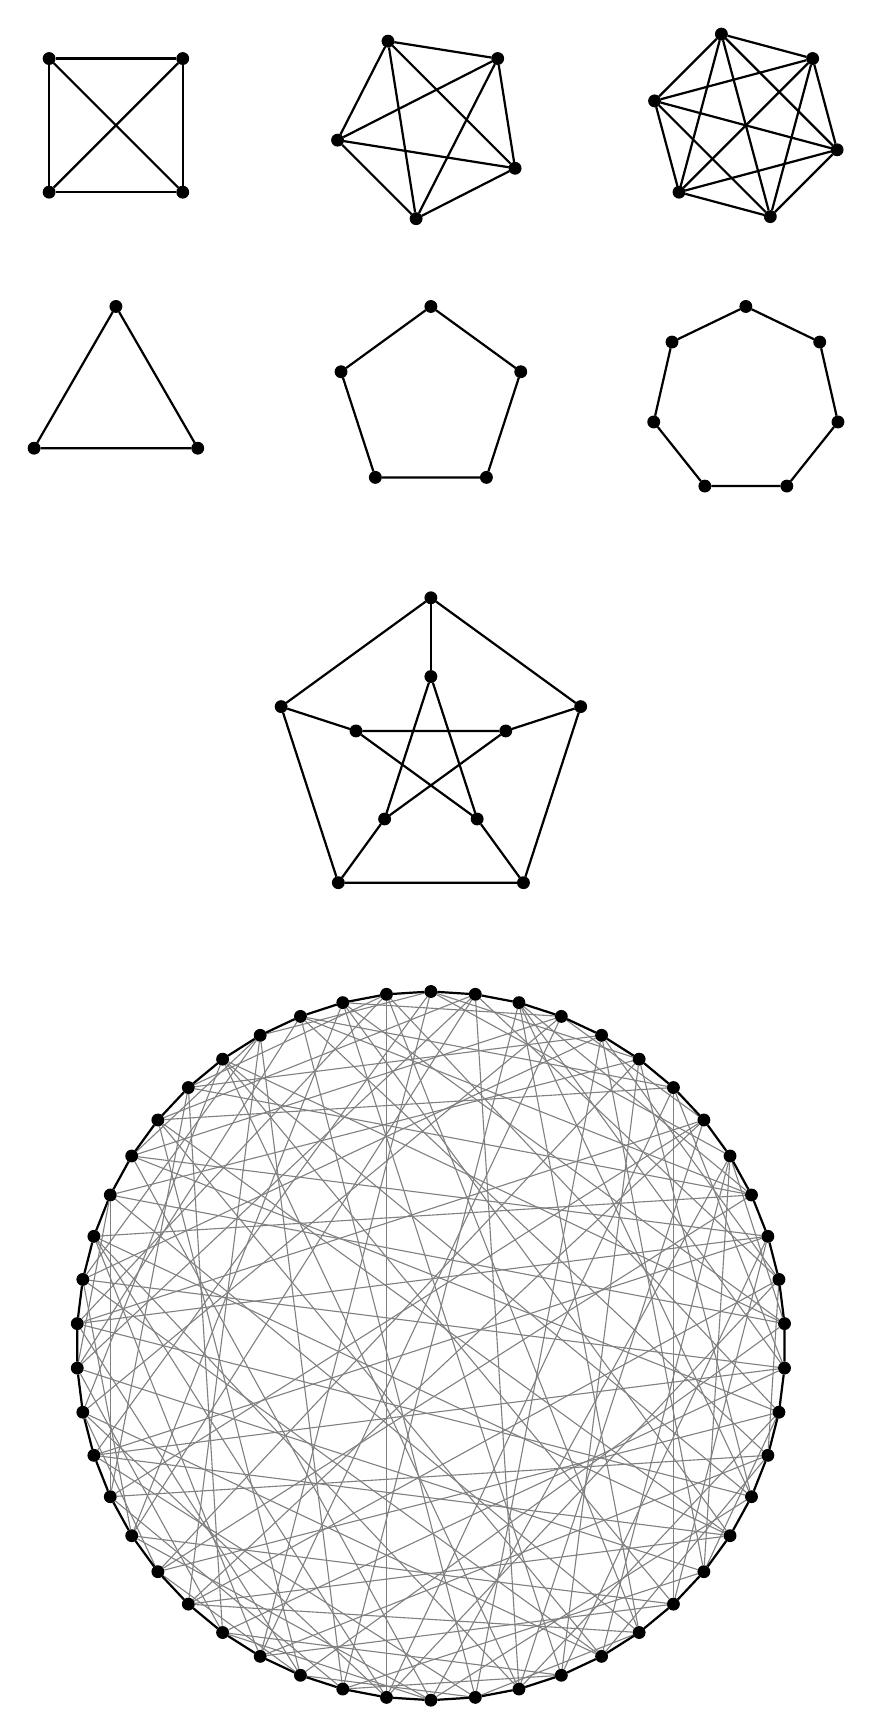
\begin{tikzpicture}[
        % Tvoji stili iz Hoffman-Singleton kode
        vnode/.style={draw, circle, fill=black, inner sep=1.5pt},
        old_edge/.style={draw, thin, gray}, % Prilagodi barvo po želji
        new_edge/.style={draw, thick, black}
    ]

        % ==========================================
        % 1. ZGORNJA VRSTA (Polni grafi)
        % ==========================================
        
        \begin{scope}[shift={(-4, 8)}]
            \foreach \i in {1,...,4} {
                \node[vnode] (k4_\i) at ({360/4 * (\i - 1) + 45}:1.2) {};
            }
            \draw[thick] (k4_1) -- (k4_2) -- (k4_3) -- (k4_4) -- (k4_1);
            \draw[thick] (k4_1) -- (k4_3);
            \draw[thick] (k4_2) -- (k4_4);
        \end{scope}
        
        \begin{scope}[shift={(0, 8)}]
            \foreach \i in {1,...,5} {
                \node[vnode] (k5_\i) at ({360/5 * (\i - 1) + 45}:1.2) {};
            }
            \foreach \i in {1,...,5}{
              \foreach \j in {1,...,5}{
                \ifnum\i<\j
                  \draw[thick] (k5_\i) -- (k5_\j);
                \fi
              }
            }
        \end{scope}
        
        \begin{scope}[shift={(4, 8)}]
            \foreach \i in {1,...,6} {
                \node[vnode] (k6_\i) at ({360/6 * (\i - 1) + 45}:1.2) {};
            }
            \foreach \i in {1,...,6}{
              \foreach \j in {1,...,6}{
                \ifnum\i<\j
                  \draw[thick] (k6_\i) -- (k6_\j);
                \fi
              }
            }
        \end{scope}

        % ==========================================
        % 2. DRUGA VRSTA (Cikli)
        % ==========================================

        % --- C_3 (Trikotnik) ---
        \begin{scope}[shift={(-4, 4.5)}]
            \foreach \i in {1,2,3} {
                \node[vnode] (c3_\i) at ({120 * (\i - 1) + 90}:1.2) {};
            }
            \draw[thick] (c3_1) -- (c3_2) -- (c3_3) -- (c3_1);
        \end{scope}

        % --- C_5 (Petkotnik) ---
        \begin{scope}[shift={(0, 4.5)}]
            \foreach \i in {1,...,5} {
                \node[vnode] (c5_\i) at ({360/5 * (\i - 1) + 90}:1.2) {};
            }
            \draw[thick] (c5_1) -- (c5_2) -- (c5_3) -- (c5_4) -- (c5_5) -- (c5_1);
        \end{scope}

        % --- C_7 (Sedemkotnik) ---
        \begin{scope}[shift={(4, 4.5)}]
            \foreach \i in {1,...,7} {
                \node[vnode] (c7_\i) at ({360/7 * (\i - 1) + 90}:1.2) {};
            }
            \draw[thick] (c7_1) -- (c7_2) -- (c7_3) -- (c7_4) -- (c7_5) -- (c7_6) -- (c7_7) -- (c7_1);
        \end{scope}
         

        % ==========================================
        % 3. SREDNJA VRSTA (Petersenov graf)
        % ==========================================

        \begin{scope}[shift={(0, 0)}]
            % Zunanji petkotnik
            \foreach \i in {1,...,5} {
                \node[vnode] (p_out_\i) at ({360/5 * (\i - 1) + 90}:2.0) {};
            }
            % Notranja zvezda
            \foreach \i in {1,...,5} {
                \node[vnode] (p_in_\i) at ({360/5 * (\i - 1) + 90}:1.0) {};
            }
            
            % Povezave zunanjega petkotnika
            \draw[thick] (p_out_1) -- (p_out_2) -- (p_out_3) -- (p_out_4) -- (p_out_5) -- (p_out_1);
            % Povezave notranje zvezde
            \draw[thick] (p_in_1) -- (p_in_3) -- (p_in_5) -- (p_in_2) -- (p_in_4) -- (p_in_1);
            % Povezave med notranjostjo in zunanjostjo
            \foreach \i in {1,...,5} {
                \draw[thick] (p_out_\i) -- (p_in_\i);
            }
        \end{scope}

        % ==========================================
        % 4. SPODNJA VRSTA (Hoffman-Singletonov graf)
        % ==========================================

        \begin{scope}[shift={(0, -7.5)}, scale=0.75, rotate=90]
           \node[vnode] (0) at (0.00:6cm) {};
  \node[vnode] (3) at (7.20:6cm) {};
  \node[vnode] (5) at (14.40:6cm) {};
  \node[vnode] (12) at (21.60:6cm) {};
  \node[vnode] (1) at (28.80:6cm) {};
  \node[vnode] (28) at (36.00:6cm) {};
  \node[vnode] (40) at (43.20:6cm) {};
  \node[vnode] (22) at (50.40:6cm) {};
  \node[vnode] (17) at (57.60:6cm) {};
  \node[vnode] (25) at (64.80:6cm) {};
  \node[vnode] (16) at (72.00:6cm) {};
  \node[vnode] (29) at (79.20:6cm) {};
  \node[vnode] (30) at (86.40:6cm) {};
  \node[vnode] (31) at (93.60:6cm) {};
  \node[vnode] (20) at (100.80:6cm) {};
  \node[vnode] (8) at (108.00:6cm) {};
  \node[vnode] (42) at (115.20:6cm) {};
  \node[vnode] (43) at (122.40:6cm) {};
  \node[vnode] (44) at (129.60:6cm) {};
  \node[vnode] (27) at (136.80:6cm) {};
  \node[vnode] (14) at (144.00:6cm) {};
  \node[vnode] (2) at (151.20:6cm) {};
  \node[vnode] (13) at (158.40:6cm) {};
  \node[vnode] (26) at (165.60:6cm) {};
  \node[vnode] (45) at (172.80:6cm) {};
  \node[vnode] (23) at (180.00:6cm) {};
  \node[vnode] (36) at (187.20:6cm) {};
  \node[vnode] (39) at (194.40:6cm) {};
  \node[vnode] (38) at (201.60:6cm) {};
  \node[vnode] (37) at (208.80:6cm) {};
  \node[vnode] (35) at (216.00:6cm) {};
  \node[vnode] (15) at (223.20:6cm) {};
  \node[vnode] (34) at (230.40:6cm) {};
  \node[vnode] (33) at (237.60:6cm) {};
  \node[vnode] (32) at (244.80:6cm) {};
  \node[vnode] (11) at (252.00:6cm) {};
  \node[vnode] (4) at (259.20:6cm) {};
  \node[vnode] (49) at (266.40:6cm) {};
  \node[vnode] (48) at (273.60:6cm) {};
  \node[vnode] (47) at (280.80:6cm) {};
  \node[vnode] (24) at (288.00:6cm) {};
  \node[vnode] (41) at (295.20:6cm) {};
  \node[vnode] (7) at (302.40:6cm) {};
  \node[vnode] (19) at (309.60:6cm) {};
  \node[vnode] (46) at (316.80:6cm) {};
  \node[vnode] (9) at (324.00:6cm) {};
  \node[vnode] (21) at (331.20:6cm) {};
  \node[vnode] (10) at (338.40:6cm) {};
  \node[vnode] (18) at (345.60:6cm) {};
  \node[vnode] (6) at (352.80:6cm) {};
  \draw[old_edge] (0) -- (1);
  \draw[old_edge] (0) -- (2);
  \draw[new_edge] (0) -- (3);
  \draw[new_edge] (0) -- (6);
  \draw[old_edge] (0) -- (7);
  \draw[old_edge] (0) -- (8);
  \draw[old_edge] (0) -- (9);
  \draw[old_edge] (1) -- (17);
  \draw[old_edge] (1) -- (26);
  \draw[old_edge] (1) -- (27);
  \draw[new_edge] (1) -- (12);
  \draw[new_edge] (1) -- (28);
  \draw[old_edge] (1) -- (29);
  \draw[old_edge] (2) -- (16);
  \draw[old_edge] (2) -- (10);
  \draw[old_edge] (2) -- (11);
  \draw[new_edge] (2) -- (13);
  \draw[new_edge] (2) -- (14);
  \draw[old_edge] (2) -- (15);
  \draw[old_edge] (3) -- (35);
  \draw[old_edge] (3) -- (4);
  \draw[new_edge] (3) -- (5);
  \draw[old_edge] (3) -- (40);
  \draw[old_edge] (3) -- (45);
  \draw[old_edge] (3) -- (30);
  \draw[old_edge] (4) -- (17);
  \draw[new_edge] (4) -- (49);
  \draw[old_edge] (4) -- (34);
  \draw[old_edge] (4) -- (39);
  \draw[new_edge] (4) -- (11);
  \draw[old_edge] (4) -- (44);
  \draw[old_edge] (5) -- (48);
  \draw[old_edge] (5) -- (33);
  \draw[old_edge] (5) -- (38);
  \draw[old_edge] (5) -- (10);
  \draw[old_edge] (5) -- (43);
  \draw[new_edge] (5) -- (12);
  \draw[new_edge] (6) -- (18);
  \draw[old_edge] (6) -- (22);
  \draw[old_edge] (6) -- (39);
  \draw[old_edge] (6) -- (43);
  \draw[old_edge] (6) -- (31);
  \draw[old_edge] (6) -- (47);
  \draw[old_edge] (7) -- (48);
  \draw[old_edge] (7) -- (34);
  \draw[new_edge] (7) -- (19);
  \draw[old_edge] (7) -- (37);
  \draw[old_edge] (7) -- (23);
  \draw[new_edge] (7) -- (41);
  \draw[old_edge] (8) -- (33);
  \draw[old_edge] (8) -- (49);
  \draw[old_edge] (8) -- (36);
  \draw[new_edge] (8) -- (20);
  \draw[old_edge] (8) -- (24);
  \draw[new_edge] (8) -- (42);
  \draw[old_edge] (9) -- (32);
  \draw[new_edge] (9) -- (21);
  \draw[old_edge] (9) -- (38);
  \draw[old_edge] (9) -- (25);
  \draw[old_edge] (9) -- (44);
  \draw[new_edge] (9) -- (46);
  \draw[old_edge] (10) -- (17);
  \draw[new_edge] (10) -- (18);
  \draw[old_edge] (10) -- (19);
  \draw[old_edge] (10) -- (20);
  \draw[new_edge] (10) -- (21);
  \draw[new_edge] (11) -- (32);
  \draw[old_edge] (11) -- (37);
  \draw[old_edge] (11) -- (42);
  \draw[old_edge] (11) -- (12);
  \draw[old_edge] (11) -- (47);
  \draw[old_edge] (12) -- (36);
  \draw[old_edge] (12) -- (41);
  \draw[old_edge] (12) -- (46);
  \draw[old_edge] (12) -- (31);
  \draw[old_edge] (13) -- (48);
  \draw[old_edge] (13) -- (36);
  \draw[old_edge] (13) -- (22);
  \draw[new_edge] (13) -- (26);
  \draw[old_edge] (13) -- (44);
  \draw[old_edge] (13) -- (30);
  \draw[old_edge] (14) -- (49);
  \draw[old_edge] (14) -- (38);
  \draw[old_edge] (14) -- (23);
  \draw[old_edge] (14) -- (40);
  \draw[new_edge] (14) -- (27);
  \draw[old_edge] (14) -- (31);
  \draw[new_edge] (15) -- (34);
  \draw[new_edge] (15) -- (35);
  \draw[old_edge] (15) -- (24);
  \draw[old_edge] (15) -- (43);
  \draw[old_edge] (15) -- (28);
  \draw[old_edge] (15) -- (46);
  \draw[old_edge] (16) -- (33);
  \draw[old_edge] (16) -- (39);
  \draw[old_edge] (16) -- (41);
  \draw[new_edge] (16) -- (25);
  \draw[old_edge] (16) -- (45);
  \draw[new_edge] (16) -- (29);
  \draw[new_edge] (17) -- (22);
  \draw[old_edge] (17) -- (23);
  \draw[old_edge] (17) -- (24);
  \draw[new_edge] (17) -- (25);
  \draw[old_edge] (18) -- (32);
  \draw[old_edge] (18) -- (49);
  \draw[old_edge] (18) -- (35);
  \draw[old_edge] (18) -- (41);
  \draw[old_edge] (18) -- (26);
  \draw[old_edge] (19) -- (39);
  \draw[old_edge] (19) -- (42);
  \draw[old_edge] (19) -- (27);
  \draw[old_edge] (19) -- (30);
  \draw[new_edge] (19) -- (46);
  \draw[old_edge] (20) -- (37);
  \draw[old_edge] (20) -- (28);
  \draw[old_edge] (20) -- (44);
  \draw[old_edge] (20) -- (45);
  \draw[new_edge] (20) -- (31);
  \draw[old_edge] (21) -- (34);
  \draw[old_edge] (21) -- (36);
  \draw[old_edge] (21) -- (40);
  \draw[old_edge] (21) -- (29);
  \draw[old_edge] (21) -- (47);
  \draw[old_edge] (22) -- (33);
  \draw[old_edge] (22) -- (37);
  \draw[new_edge] (22) -- (40);
  \draw[old_edge] (22) -- (46);
  \draw[old_edge] (23) -- (32);
  \draw[new_edge] (23) -- (36);
  \draw[old_edge] (23) -- (43);
  \draw[new_edge] (23) -- (45);
  \draw[old_edge] (24) -- (38);
  \draw[new_edge] (24) -- (41);
  \draw[old_edge] (24) -- (30);
  \draw[new_edge] (24) -- (47);
  \draw[old_edge] (25) -- (48);
  \draw[old_edge] (25) -- (35);
  \draw[old_edge] (25) -- (42);
  \draw[old_edge] (25) -- (31);
  \draw[old_edge] (26) -- (34);
  \draw[old_edge] (26) -- (38);
  \draw[old_edge] (26) -- (42);
  \draw[new_edge] (26) -- (45);
  \draw[old_edge] (27) -- (33);
  \draw[old_edge] (27) -- (35);
  \draw[new_edge] (27) -- (44);
  \draw[old_edge] (27) -- (47);
  \draw[old_edge] (28) -- (32);
  \draw[old_edge] (28) -- (48);
  \draw[old_edge] (28) -- (39);
  \draw[new_edge] (28) -- (40);
  \draw[old_edge] (29) -- (49);
  \draw[old_edge] (29) -- (37);
  \draw[old_edge] (29) -- (43);
  \draw[new_edge] (29) -- (30);
  \draw[old_edge] (30) -- (32);
  \draw[new_edge] (30) -- (31);
  \draw[old_edge] (31) -- (34);
  \draw[new_edge] (32) -- (33);
  \draw[new_edge] (33) -- (34);
  \draw[old_edge] (35) -- (36);
  \draw[new_edge] (35) -- (37);
  \draw[new_edge] (36) -- (39);
  \draw[new_edge] (37) -- (38);
  \draw[new_edge] (38) -- (39);
  \draw[old_edge] (40) -- (41);
  \draw[old_edge] (40) -- (42);
  \draw[old_edge] (41) -- (44);
  \draw[new_edge] (42) -- (43);
  \draw[new_edge] (43) -- (44);
  \draw[old_edge] (45) -- (46);
  \draw[old_edge] (45) -- (47);
  \draw[old_edge] (46) -- (49);
  \draw[new_edge] (47) -- (48);
  \draw[new_edge] (48) -- (49);
            
        \end{scope}

    \end{tikzpicture}